%%
% The BIThesis Template for Presentation
%
% 北京理工大学毕业设计(论文) —— 使用 XeLaTeX 编译
%
% Copyright 2021-2022 BITNP
%
% This work may be distributed and/or modified under the
% conditions of the LaTeX Project Public License, either version 1.3
% of this license or (at your option) any later version.
% The latest version of this license is in
%   http://www.latex-project.org/lppl.txt
% and version 1.3 or later is part of all distributions of LaTeX
% version 2005/12/01 or later.
%
% This work has the LPPL maintenance status `maintained'.
%
% The Current Maintainer of this work is Feng Kaiyu.
%
% Compile with: xelatex -> biber -> xelatex -> xelatex
%%

\documentclass[
  %% ====== 这一部分选项将传递给 ctexbeamer,你也可以添加其他的选项 ====
  % 修改 `aspectratio` 可以修改画布比例 比如 `43` 或者 `169`
  aspectratio=169,
  presentation,
  %% ============================================================
  % 设置封面的图片
  titlegraphic=./images/bit.png,
  % 设置每页标题的 logo
  framelogo=./images/bit.png
]{bitbeamer}

%% --> 基本信息设置
\title{从 BIT-Thesis 到 BIThesis}
\subtitle{助力北理学子高质量学术写作}
\author{冯开宇}
\institute{北京理工大学}
\date{\zhdate{2023/02/22}}

\usefonttheme{serif}              % 使用衬线字体
\usefonttheme{professionalfonts}  % 数学公式字体

% 引入你需要使用的包
\usepackage{caption}
\usepackage{subcaption}
\usepackage{color}
\usepackage{listings}

\setbeamertemplate{caption}[numbered]

% 使用 bibtex
\usepackage[
  backend=biber,
  style=gb7714-2015,
  gbalign=gb7714-2015,
  gbnamefmt=lowercase,
  gbpub=false,
  doi=false,
  url=false,
  eprint=false,
  isbn=false,
]{biblatex}

\addbibresource{ref.bib}

% 设置段落间距
\parindent2em

\begin{document}

% 封面
\frame{\titlepage}

%
%% --> 目录结构
%
\begin{frame}{目录}
  \tableofcontents[hideallsubsections]
\end{frame}

%% 每一节开头显示目录,并高亮当前节的主题
\AtBeginSection[]{\frame{\tableofcontents[currentsection,hideallsubsections]}}

\section{BIThesis 项目简介}

\begin{frame}[t]
  \frametitle{BIThesis 项目简介}
  BIThesis \textbf{从 2019 年开始提供北理工本科毕设的 LaTeX 模板}。
  在后续的更新和维护中,BIThesis 也提供了本科全英文专业毕设模板、本科毕设外文翻译模板、计算机学院开题报告等等模板。

  去年,BIThesis \textbf{从 BIT-Thesis 项目中迁移了研究生学位论文模板}。
  并在去年暑假期间,针对同学们的现有反馈,
  \textbf{对模板进行了重写,使得模板更加易用},更加符合北理工的毕设要求。

  \vspace{0.5cm}

  排版样式参考:
  \begin{enumerate}
    \item 《北京理工大学研究生学位论文撰写规范》
    \item \href{https://grd.bit.edu.cn/xwgz/xwgz2/wjxz_xwgz/b119746.htm}{研究生学位论文模版 Word 版本 - 2018}
    \item BIT-Thesis 项目
    \item 部分同学的反馈与日常使用习惯
  \end{enumerate}
\end{frame}




%% --> 正式内容开始
%
\section{BIThesis 相比原有项目有什么优点?}    % 第 1 节

\begin{frame}[t] % 第一页
  \frametitle{BIThesis 相比原有项目有什么优点?}

  \begin{itemize}
    \item 使用 LaTeX3,提供给用户更灵活、强大的配置能力。
    \item 修复了原有项目中的一些细节问题。
    \item 更接近《北京理工大学研究生学位论文撰写规范》。
    \item 持续维护的项目。
  \end{itemize}
\end{frame}

\begin{frame}[fragile]
  \frametitle{BIThesis 相比原有项目有什么优点?}
  \framesubtitle{使用 LaTeX3,提供给用户更灵活、强大的配置能力}

  \vspace{-0.6cm}

  \begin{figure}
    \begin{center}
      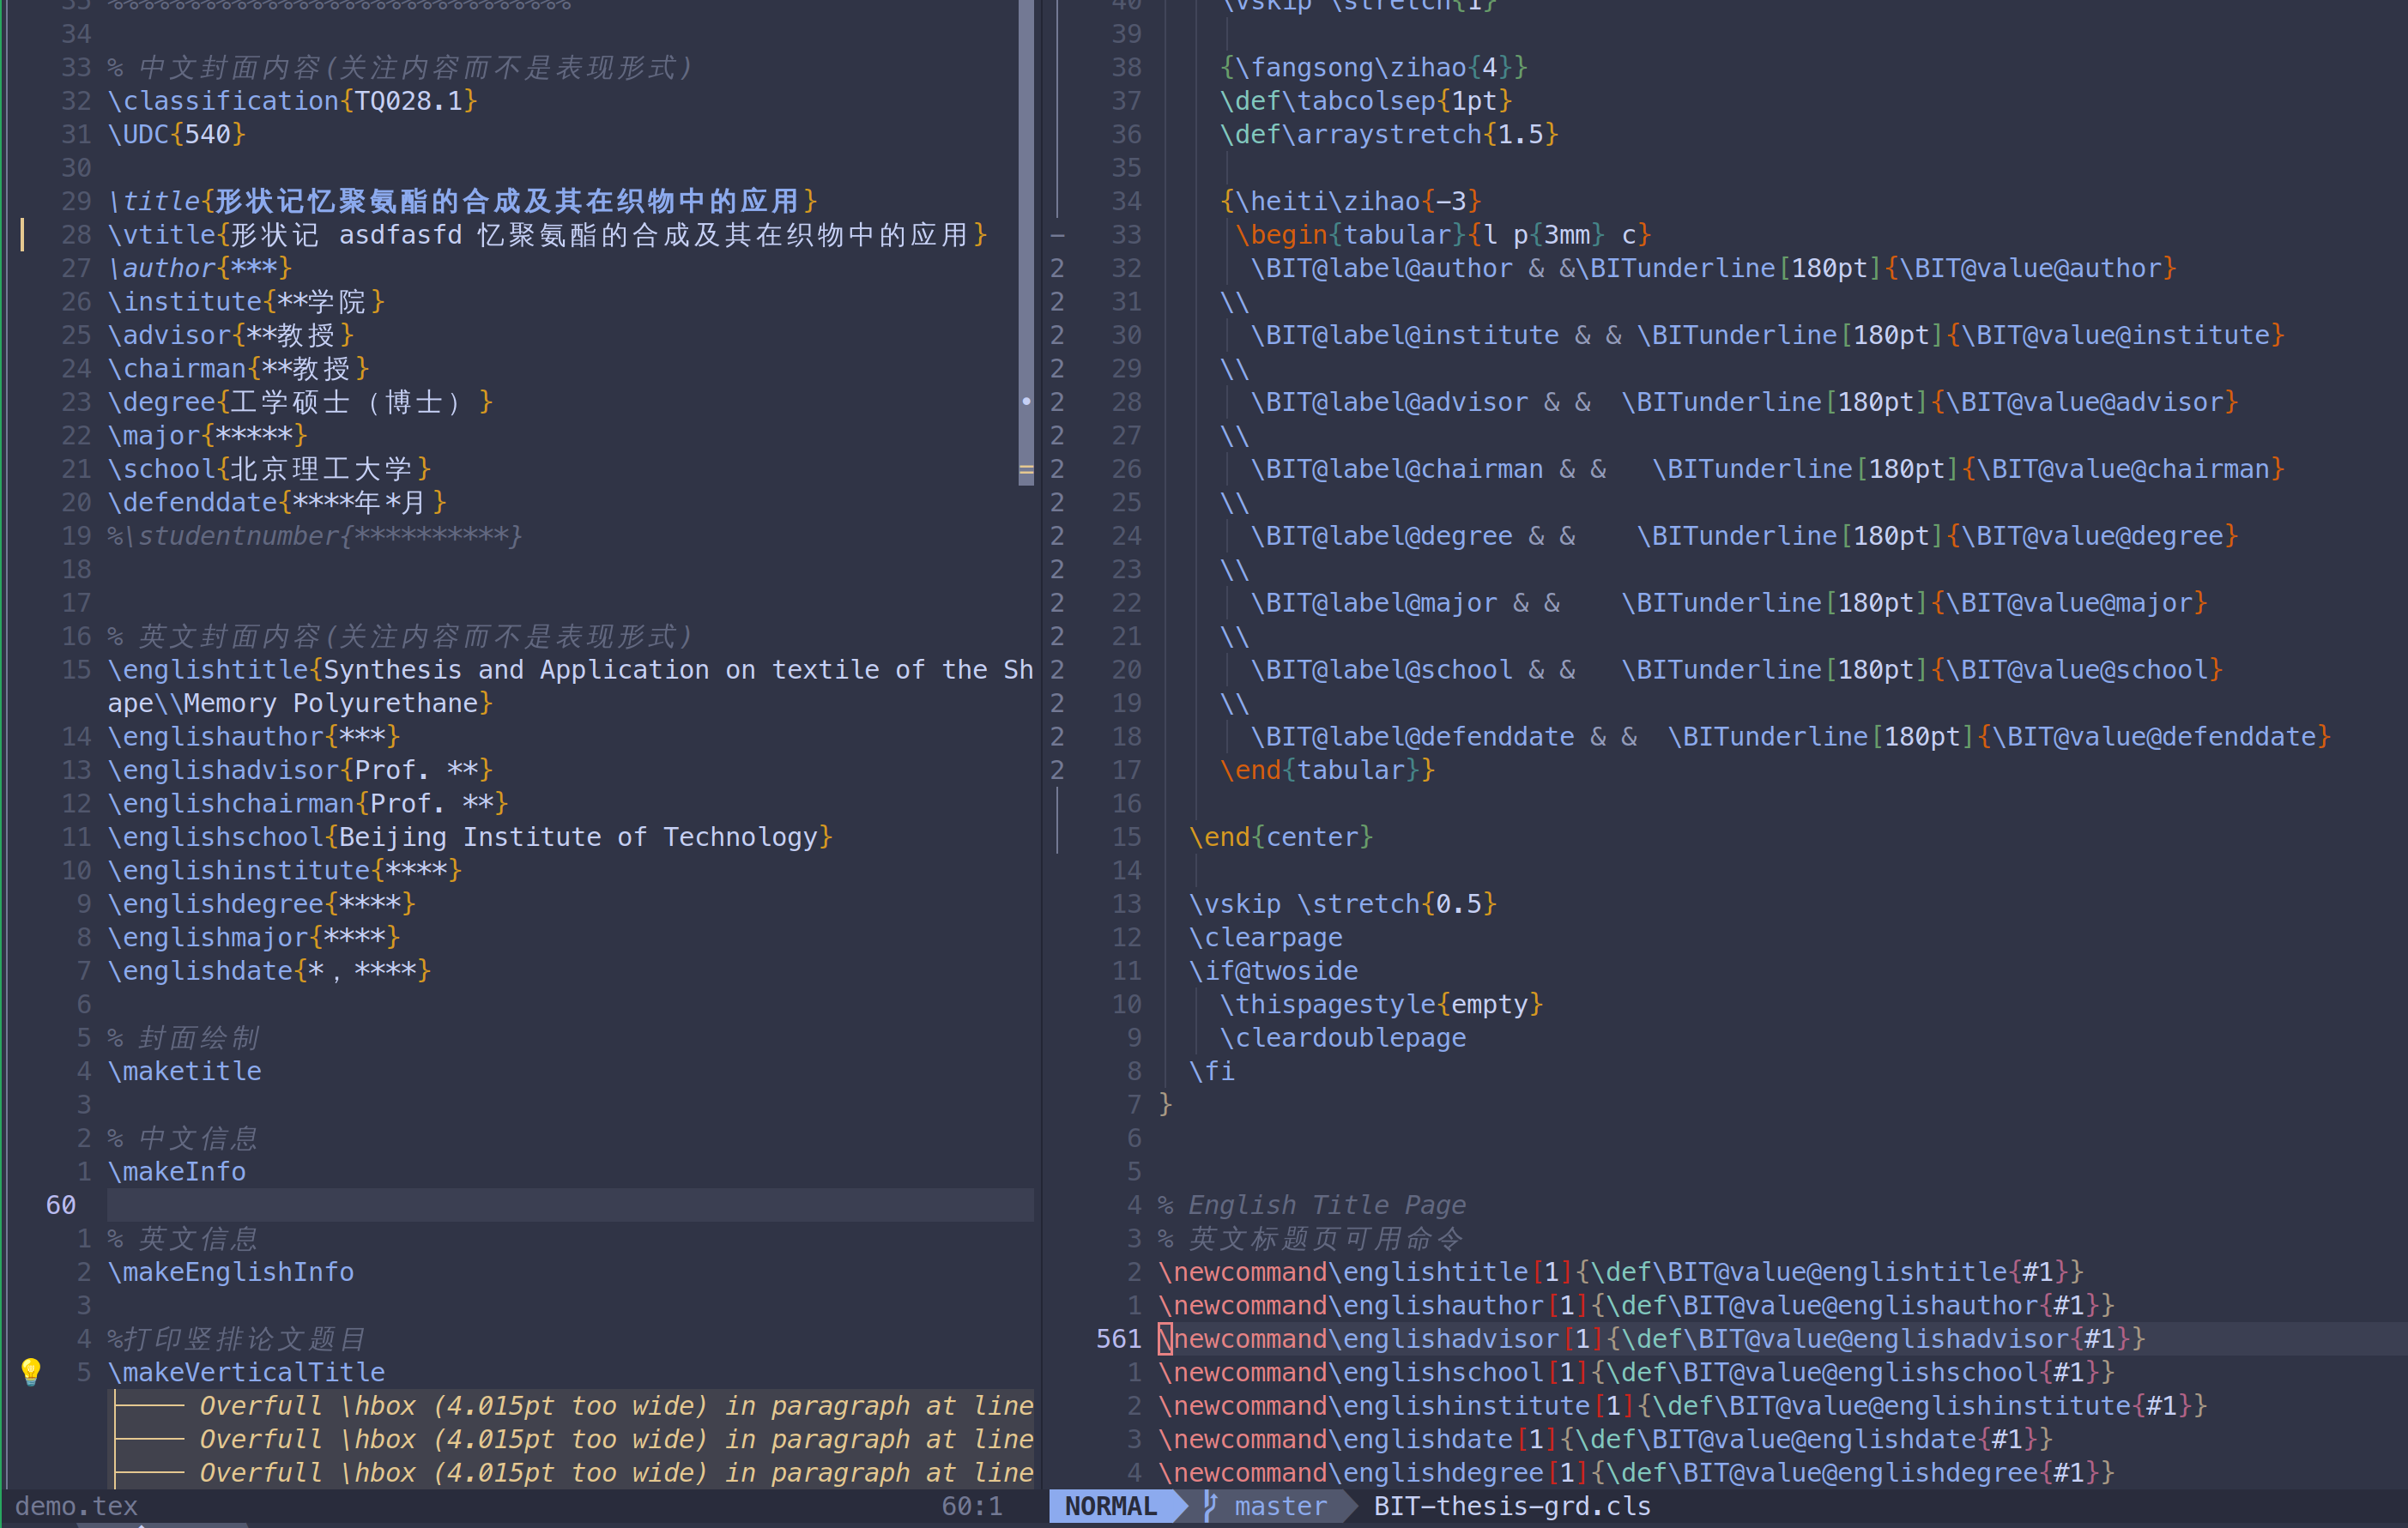
\includegraphics[width=0.63\textwidth]{images/4.png}
    \end{center}
    \caption{原项目的配置方式:可以录入信息,但无法方便地控制样式}
  \end{figure}
\end{frame}

\begin{frame}[t]
  \frametitle{BIThesis 相比原有项目有什么优点?}
  \framesubtitle{使用 LaTeX3,提供给用户更灵活、强大的配置能力}
  
  \vspace{-0.8cm}

  \begin{figure}
    \begin{center}
      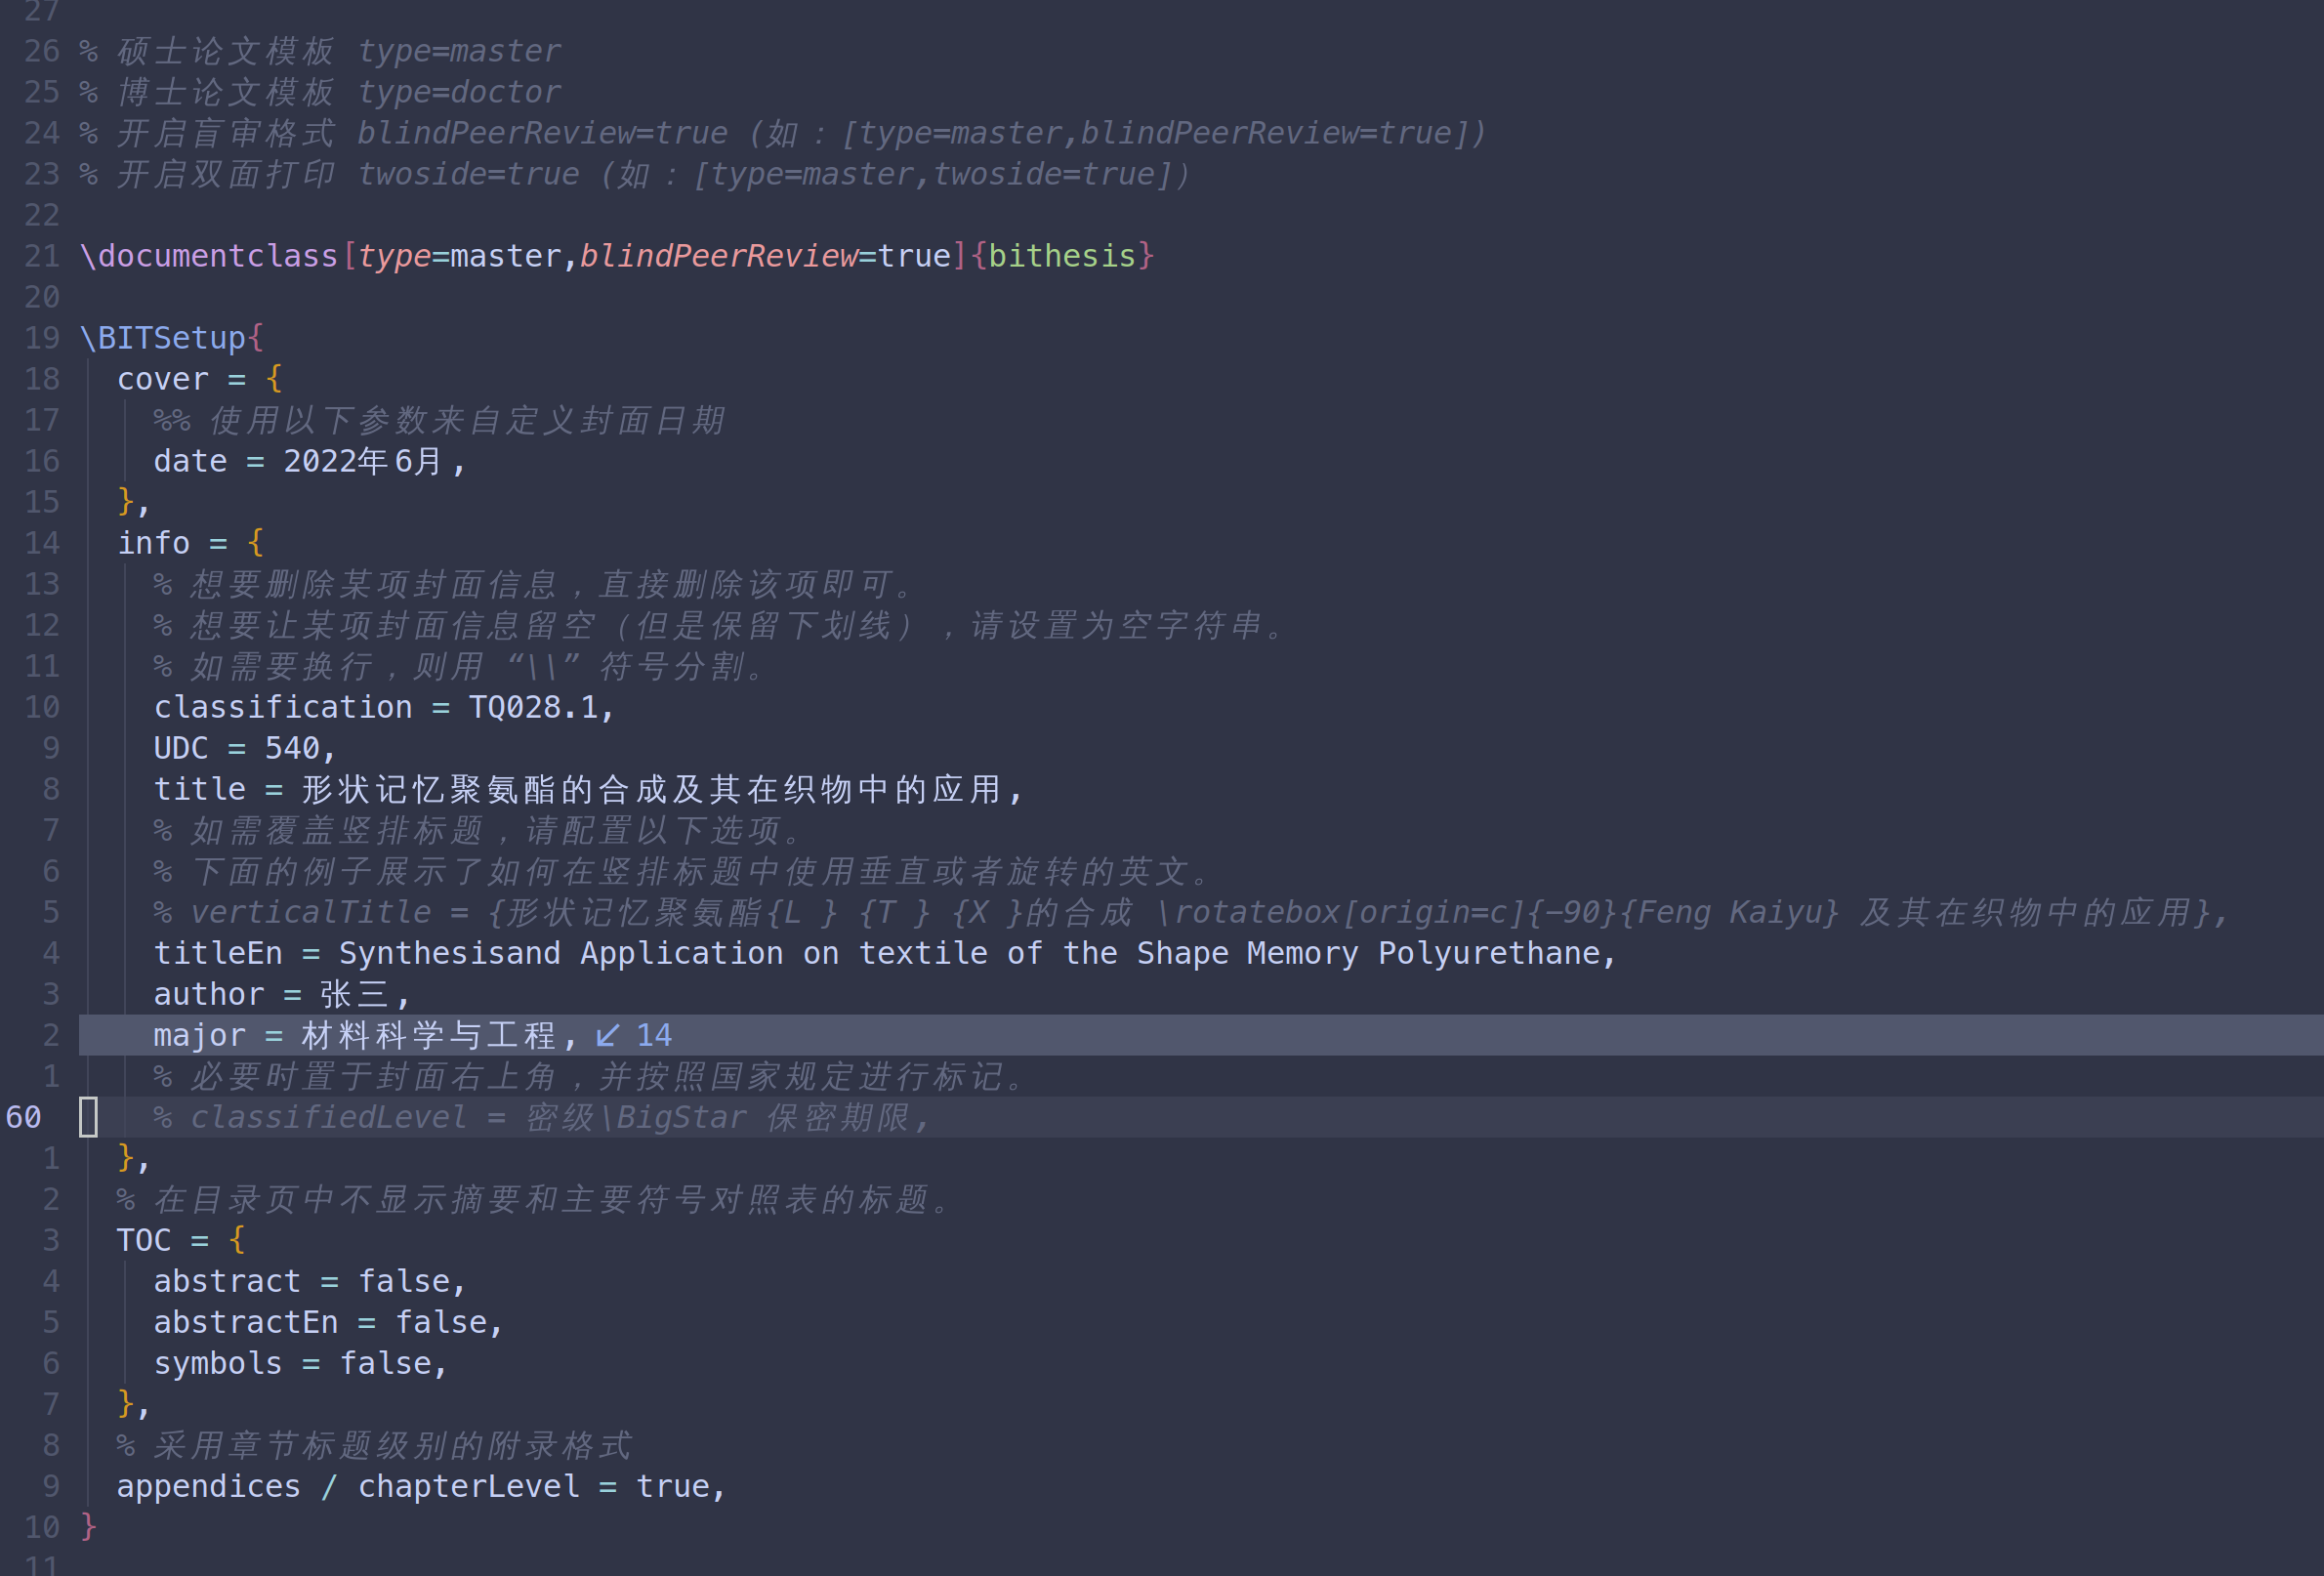
\includegraphics[width=0.6\textwidth]{./images/1.png}
    \end{center}
    \caption{新项目的配置方式:同时包括信息录入和样式控制(选项作用均在手册中记录)}
  \end{figure}
  
\end{frame}


\begin{frame}[t]
  \frametitle{BIThesis 相比原有项目有什么优点?}
  \framesubtitle{修复原有细节问题}

  原项目已经是一个非常优秀的项目了;但是在使用过程中,同学们先后反馈了许多细节上的建议。
  % \begin{itemize}
  %   \item 书脊页竖排,没有考虑到存在英文的情况。
  %   \begin{itemize}
  %     \item 针对英文单词,提供了 90 度旋转排版方案。
  %     \item 针对英文缩写,采用竖排方案。
  %   \end{itemize}
  %   \item 封面个人信息项的下划线采用了固定长度,没有兼顾到不同内容长度。
  %   \begin{itemize}
  %     \item 模板会自动按照最长信息长度,自动计算下划线长度。
  %     \item 提供了换行排版的方式。
  %   \end{itemize}
  %   \item 没有提供盲审功能。
  %   \begin{itemize}
  %     \item 可以通过选项开启盲审功能,此时生成的论文将按照盲审格式,隐去存在个人信息的部分。
  %   \end{itemize}
  %   \item 目录页出现“摘要”的索引。
  %   \begin{itemize}
  %     \item 默认情况下,不显示“摘要”。
  %     \item 用户可以通过选项自行打开。
  %   \end{itemize}
  % \end{itemize}
\end{frame}

\begin{frame}[t]
  \frametitle{BIThesis 相比原有项目有什么优点?}
  \framesubtitle{修复原有细节问题: 例1 书脊页竖排}

  \vspace{-0.8cm}

  \begin{figure}
    \begin{subfigure}{0.45\textwidth}
      
\includegraphics[width=0.9\textwidth]{images/5-1.png}
    \end{subfigure}
    \begin{subfigure}{0.45\textwidth}
      
\includegraphics[width=0.9\textwidth]{images/5-2.png}
    \end{subfigure}
  \end{figure}
  
\end{frame}

\begin{frame}[t]
  \frametitle{BIThesis 相比原有项目有什么优点?}
  \framesubtitle{修复原有细节问题: 例2 自适应的下划线长度}

  \vspace{-0.8cm}

  \begin{figure}
    \begin{subfigure}{0.45\textwidth}
      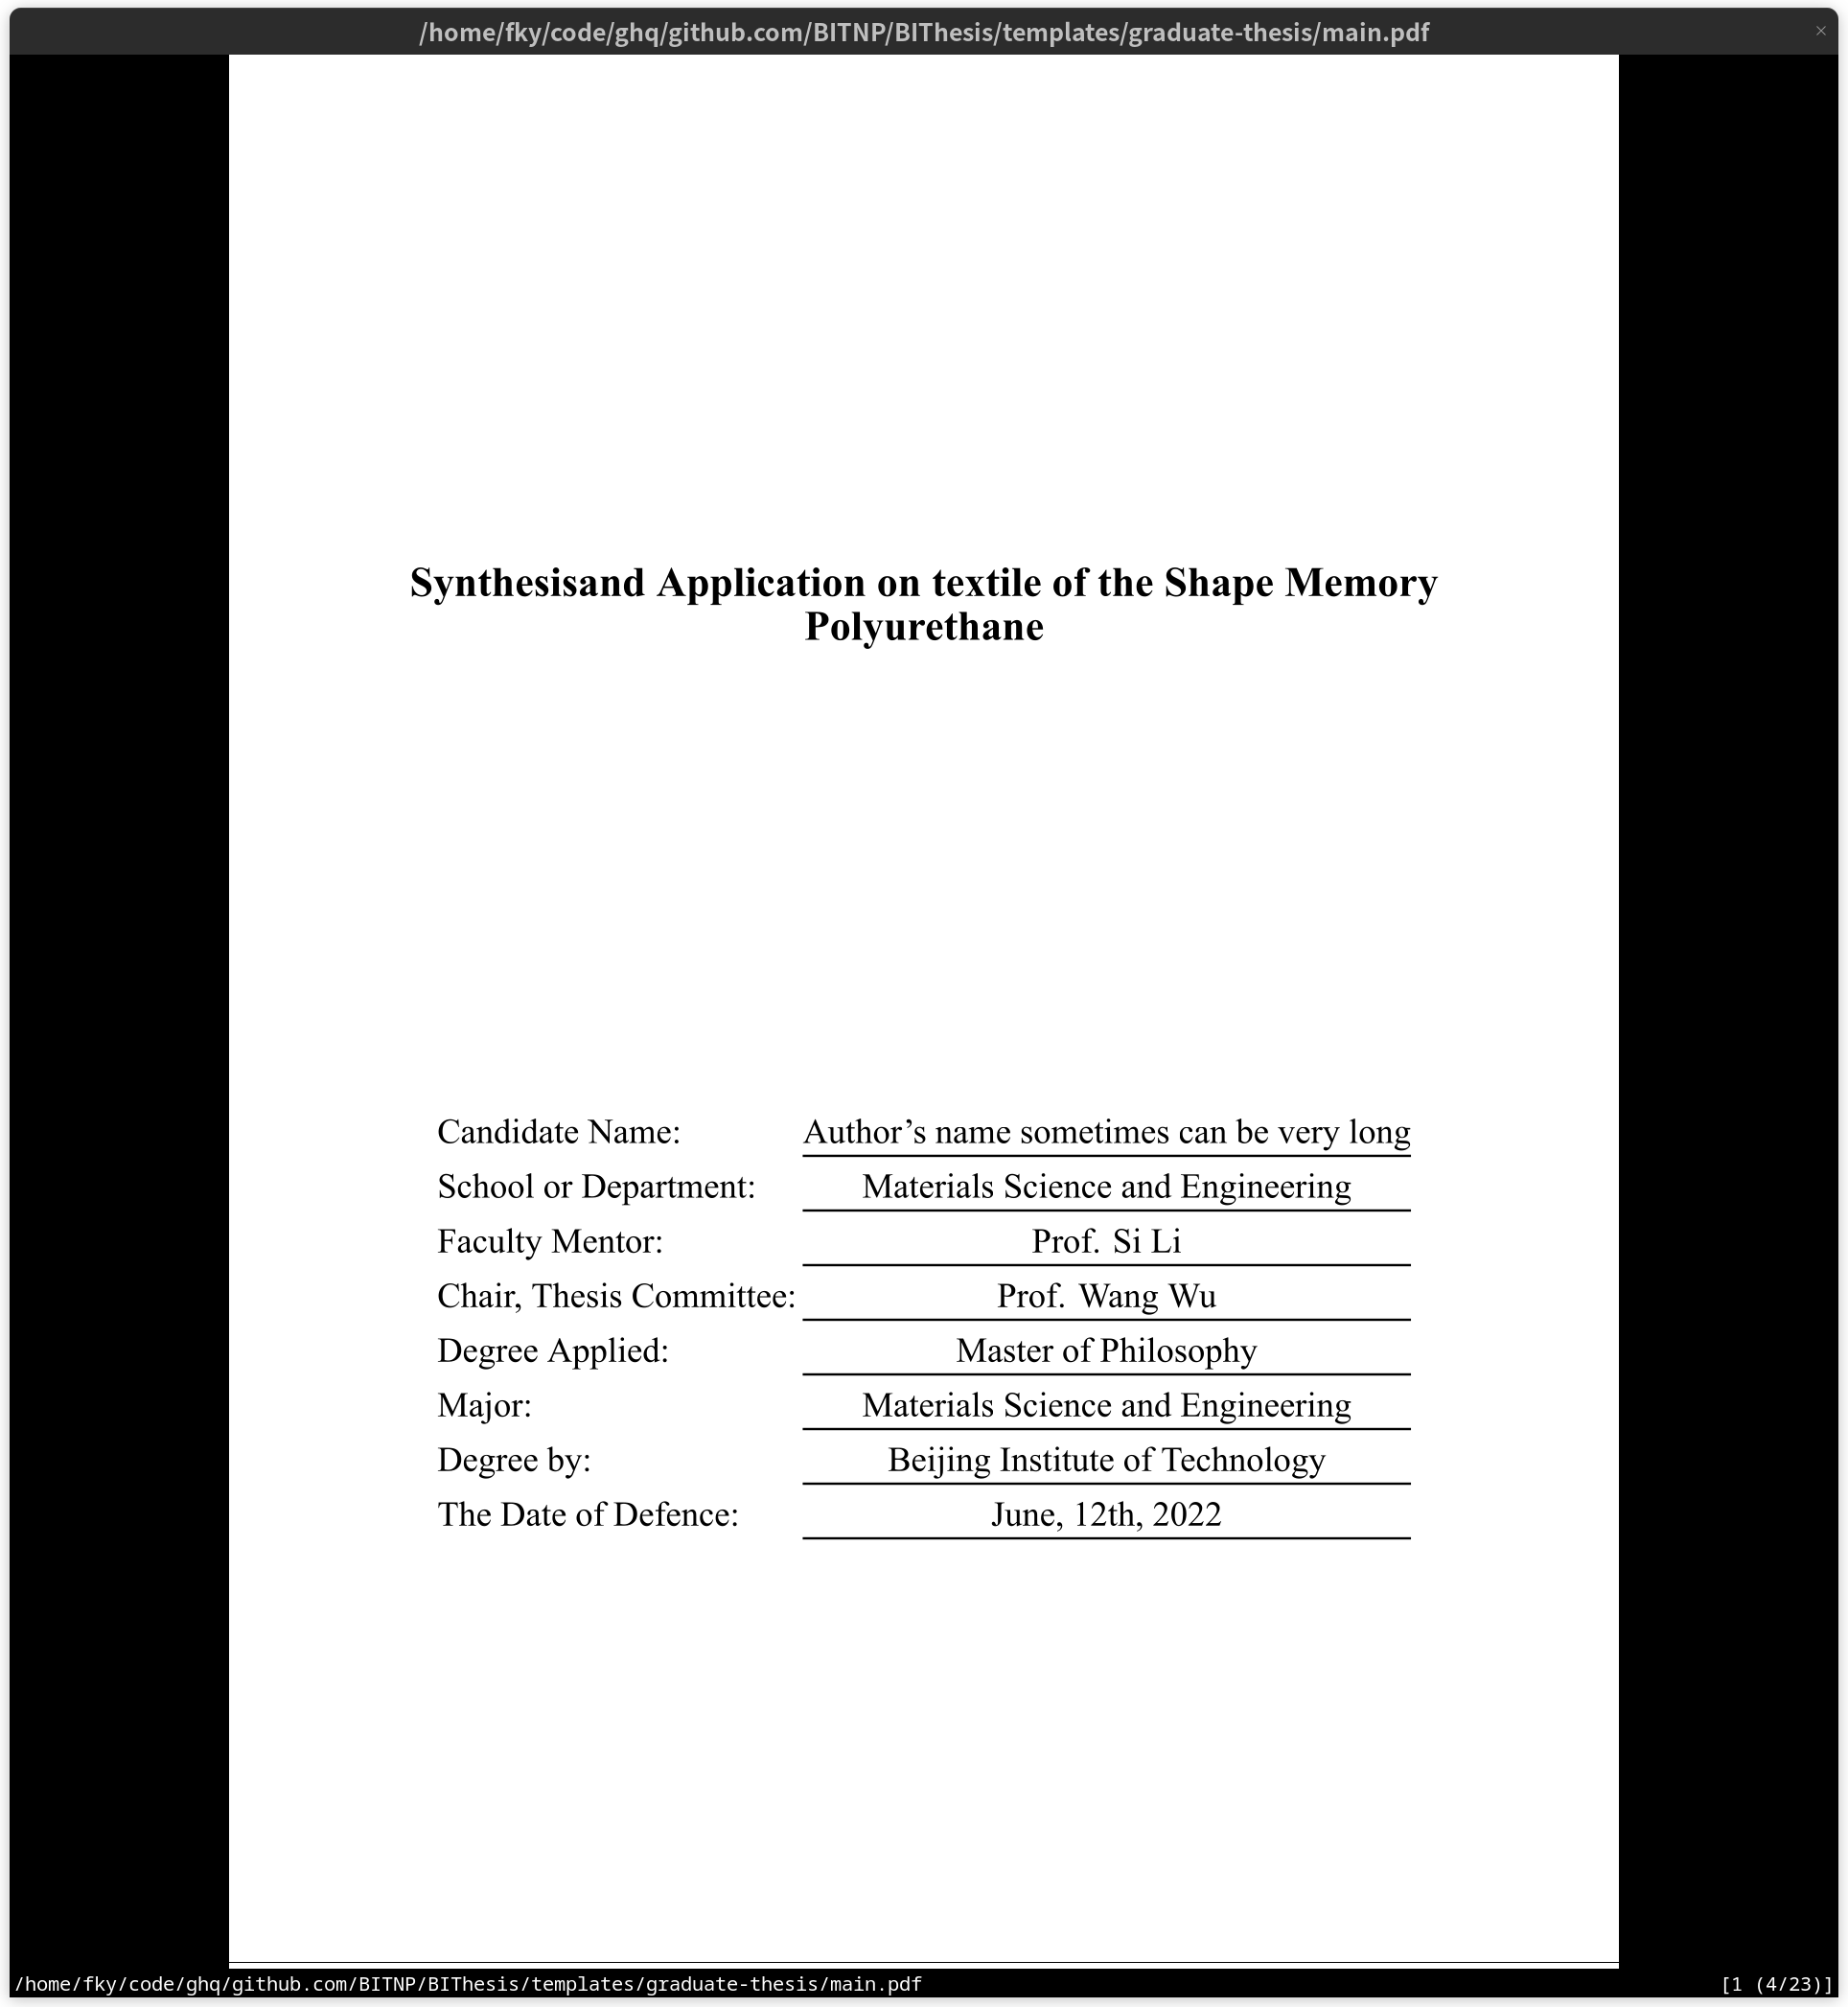
\includegraphics[width=0.9\textwidth]{images/6-1.png}
    \end{subfigure}
    \begin{subfigure}{0.45\textwidth}
      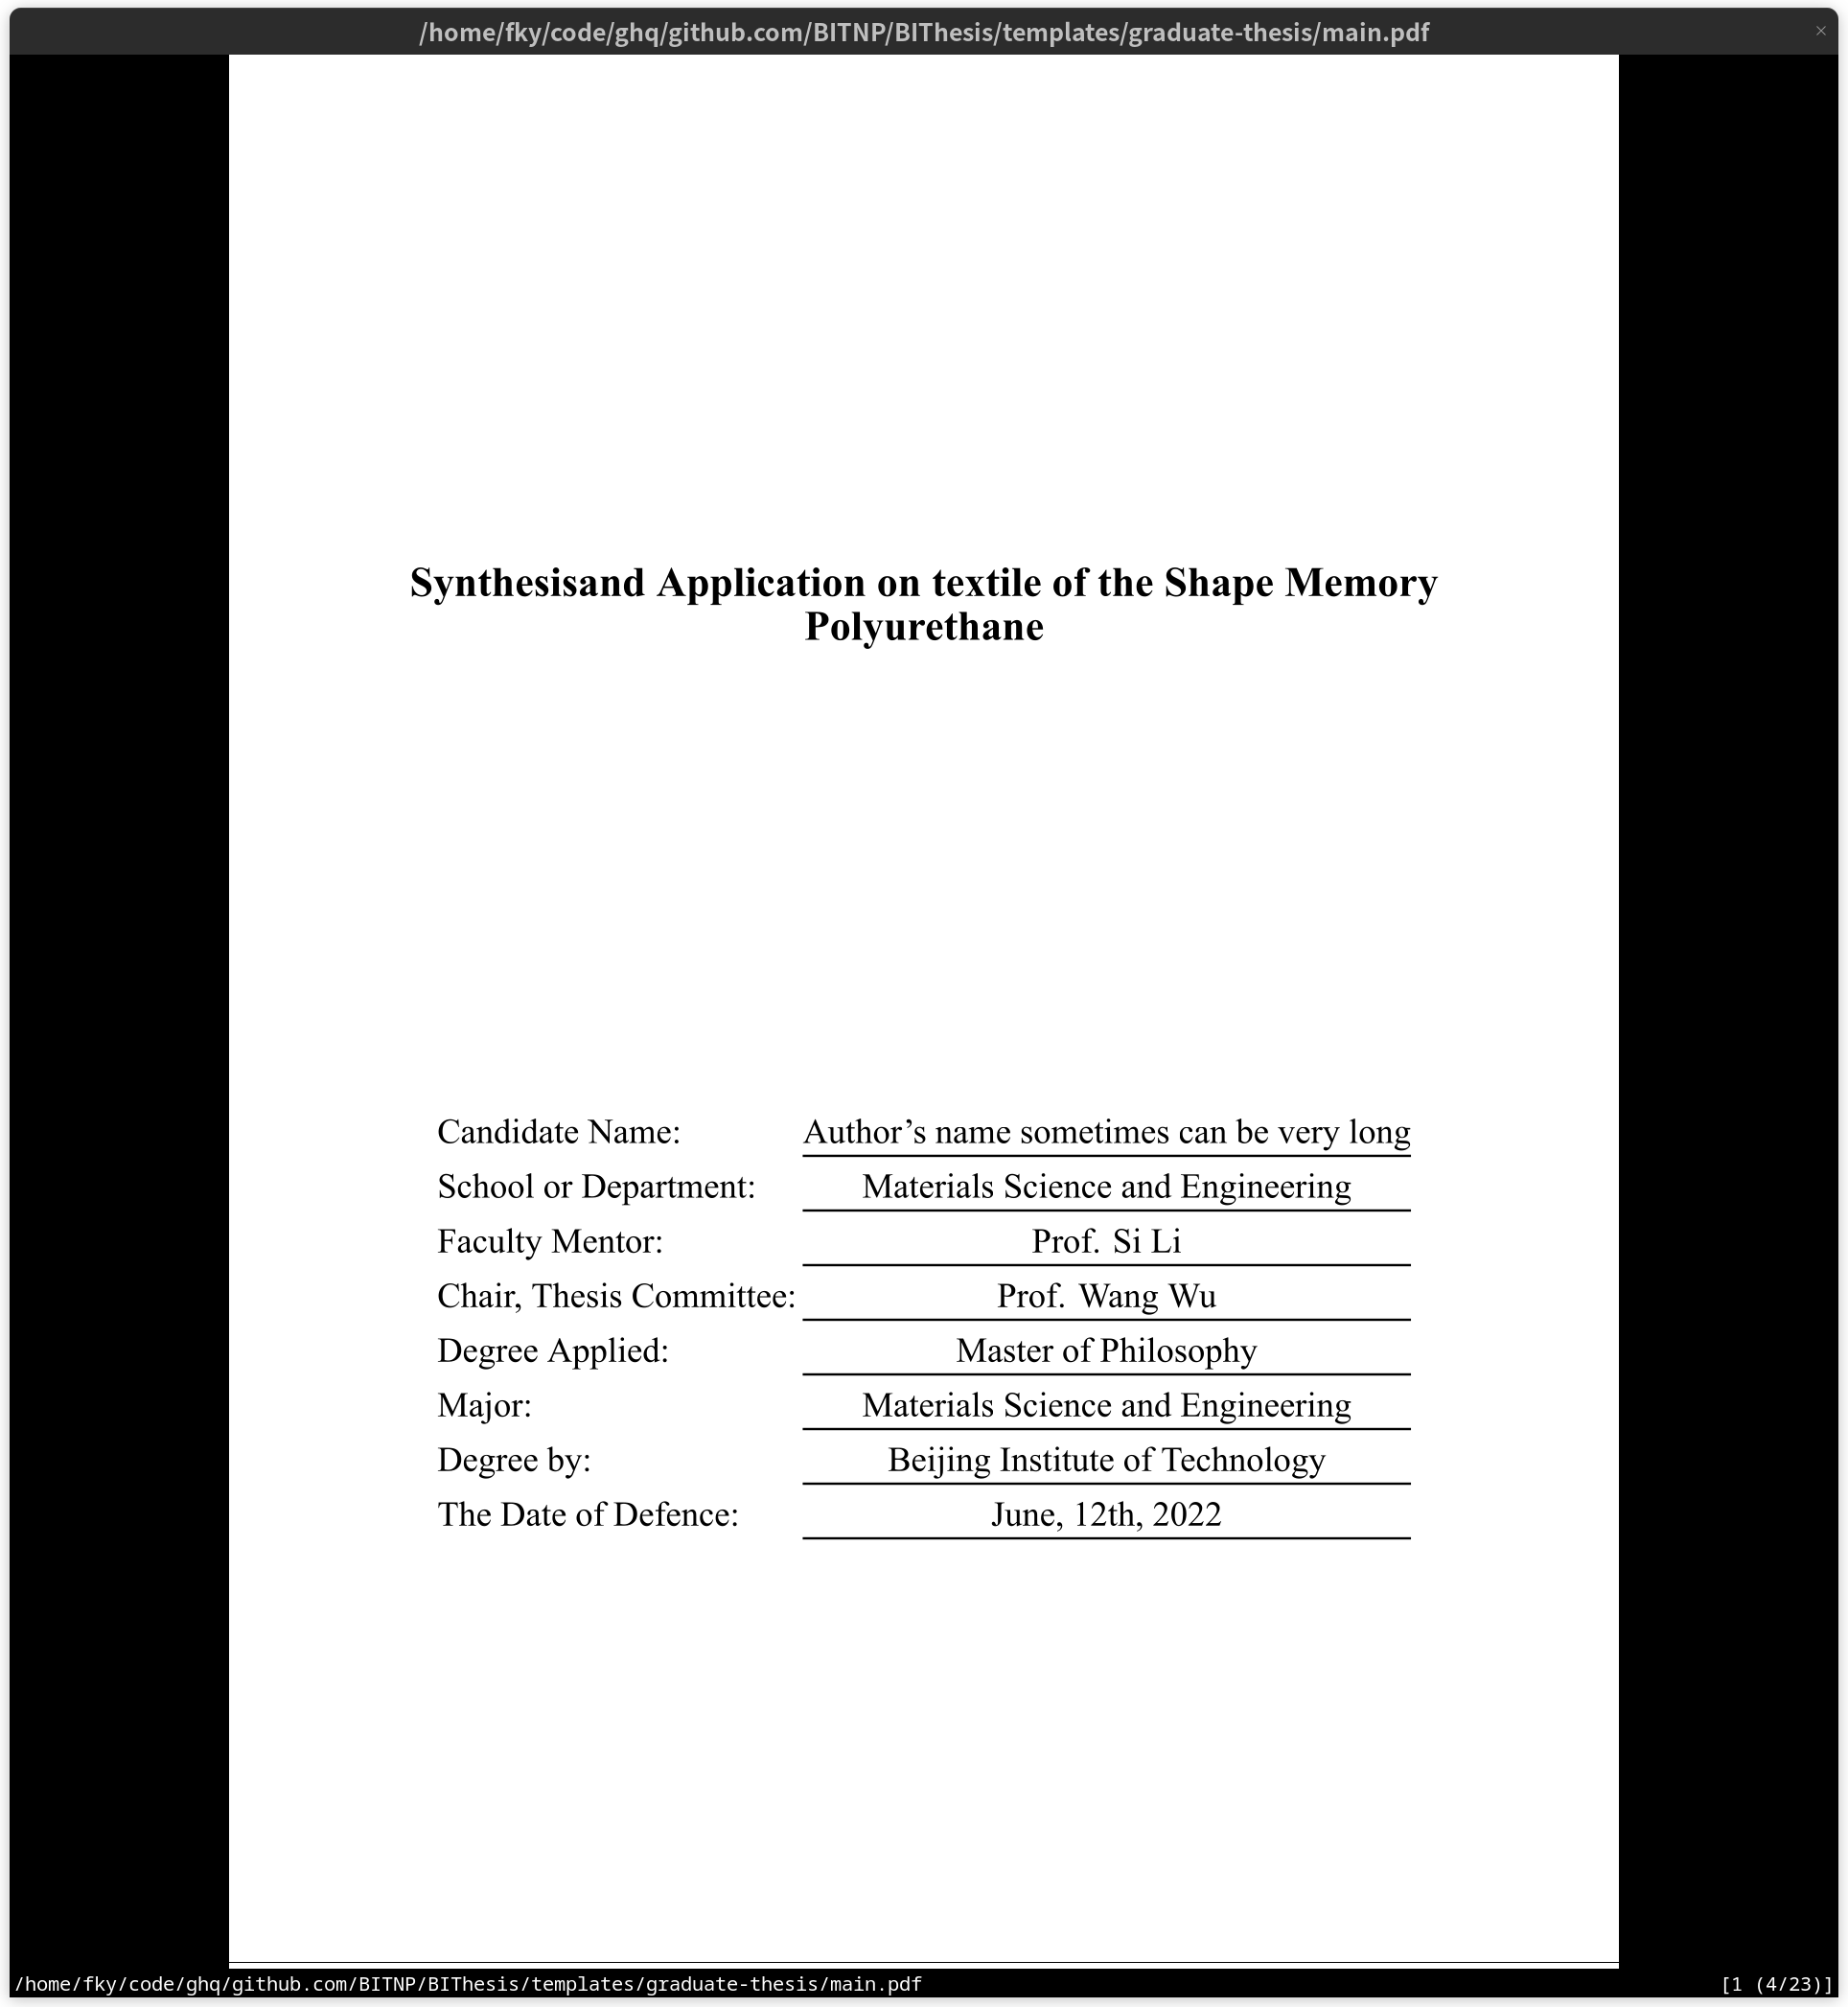
\includegraphics[width=0.9\textwidth]{images/6-2.png}
    \end{subfigure}
  \end{figure}
\end{frame}



\begin{frame}[t]
  \frametitle{BIThesis 相比原有项目有什么优点?}
  \framesubtitle{修复原有细节问题: 例3 一键导出盲审格式}

  \vspace{-0.8cm}

  \begin{figure}
    \begin{subfigure}{0.45\textwidth}
      
\includegraphics[width=0.9\textwidth]{images/7-1.png}
    \end{subfigure}
    \begin{subfigure}{0.45\textwidth}
      
\includegraphics[width=0.9\textwidth]{images/7-2.png}
    \end{subfigure}
  \end{figure}
\end{frame}


\begin{frame}[t]
  \frametitle{BIThesis 相比原有项目有什么优点?}
  \framesubtitle{更接近《北京理工大学研究生学位论文撰写规范》}

  \begin{itemize}
    \item BIThesis \textbf{首先保证论文的格式符合《北京理工大学研究生学位论文撰写规范》}。
    \item 对于没有规定的内容,BIThesis 会\textbf{尽可能地保持与原有项目的一致性}。
    \item 对于存在自定义空间的部分,BIThesis 会提供\textbf{多种选项}(以及文档),让用户自行选择。
  \end{itemize}
  

\end{frame}

\begin{frame}[t]
  \frametitle{BIThesis 相比原有项目有什么优点?}
  \framesubtitle{持续维护的项目}

  BIThesis 目前包括多种访问渠道:
  \begin{itemize}
    \item 项目主页 \url{https://bithesis.bitnp.net}
    \item 项目源代码仓库 \url{https://github.com/BITNP/BIThesis}
    \item 项目使用手册 (附于用户下载的文件中)
  \end{itemize}

  \vspace{0.5cm}
  
  项目已受到大量使用:
  \begin{itemize}
    \item 4000 余次下载量。(包含其他模板下载量)
    \item 15 名贡献者先后参与贡献代码,以及更多同学提供意见和建议。
    \item 有 QQ 交流社区。
    \item \textbf{完整的文档、测试和发布流程}。
  \end{itemize}
\end{frame}

\section{BIThesis 的维护以及其他服务}

\begin{frame}[t]
  \frametitle{BIThesis 的维护以及其他服务}
  \framesubtitle{用户可以通过\textbf{多种渠道}使用 BIThesis}

\begin{itemize}
  \item 可以通过 Github Release 下载最新的模板压缩包。
  \item 可以通过 Overleaf 平台,进行\textbf{在线的 \LaTeX 写作}。
  \item BIThesis 的模板样式已经发布到 CTAN 中,用户可以直接引入后使用。(只要安装了 \LaTeX (发行版)的用户,可以在不用下载模板的情况下直接开始写作)
\end{itemize}
\end{frame}

\begin{frame}[c]
  \frametitle{BIThesis 的维护以及其他服务}
  \framesubtitle{多种测试方法}

\begin{figure}
    \centering
    \begin{subfigure}{0.49\textwidth}
      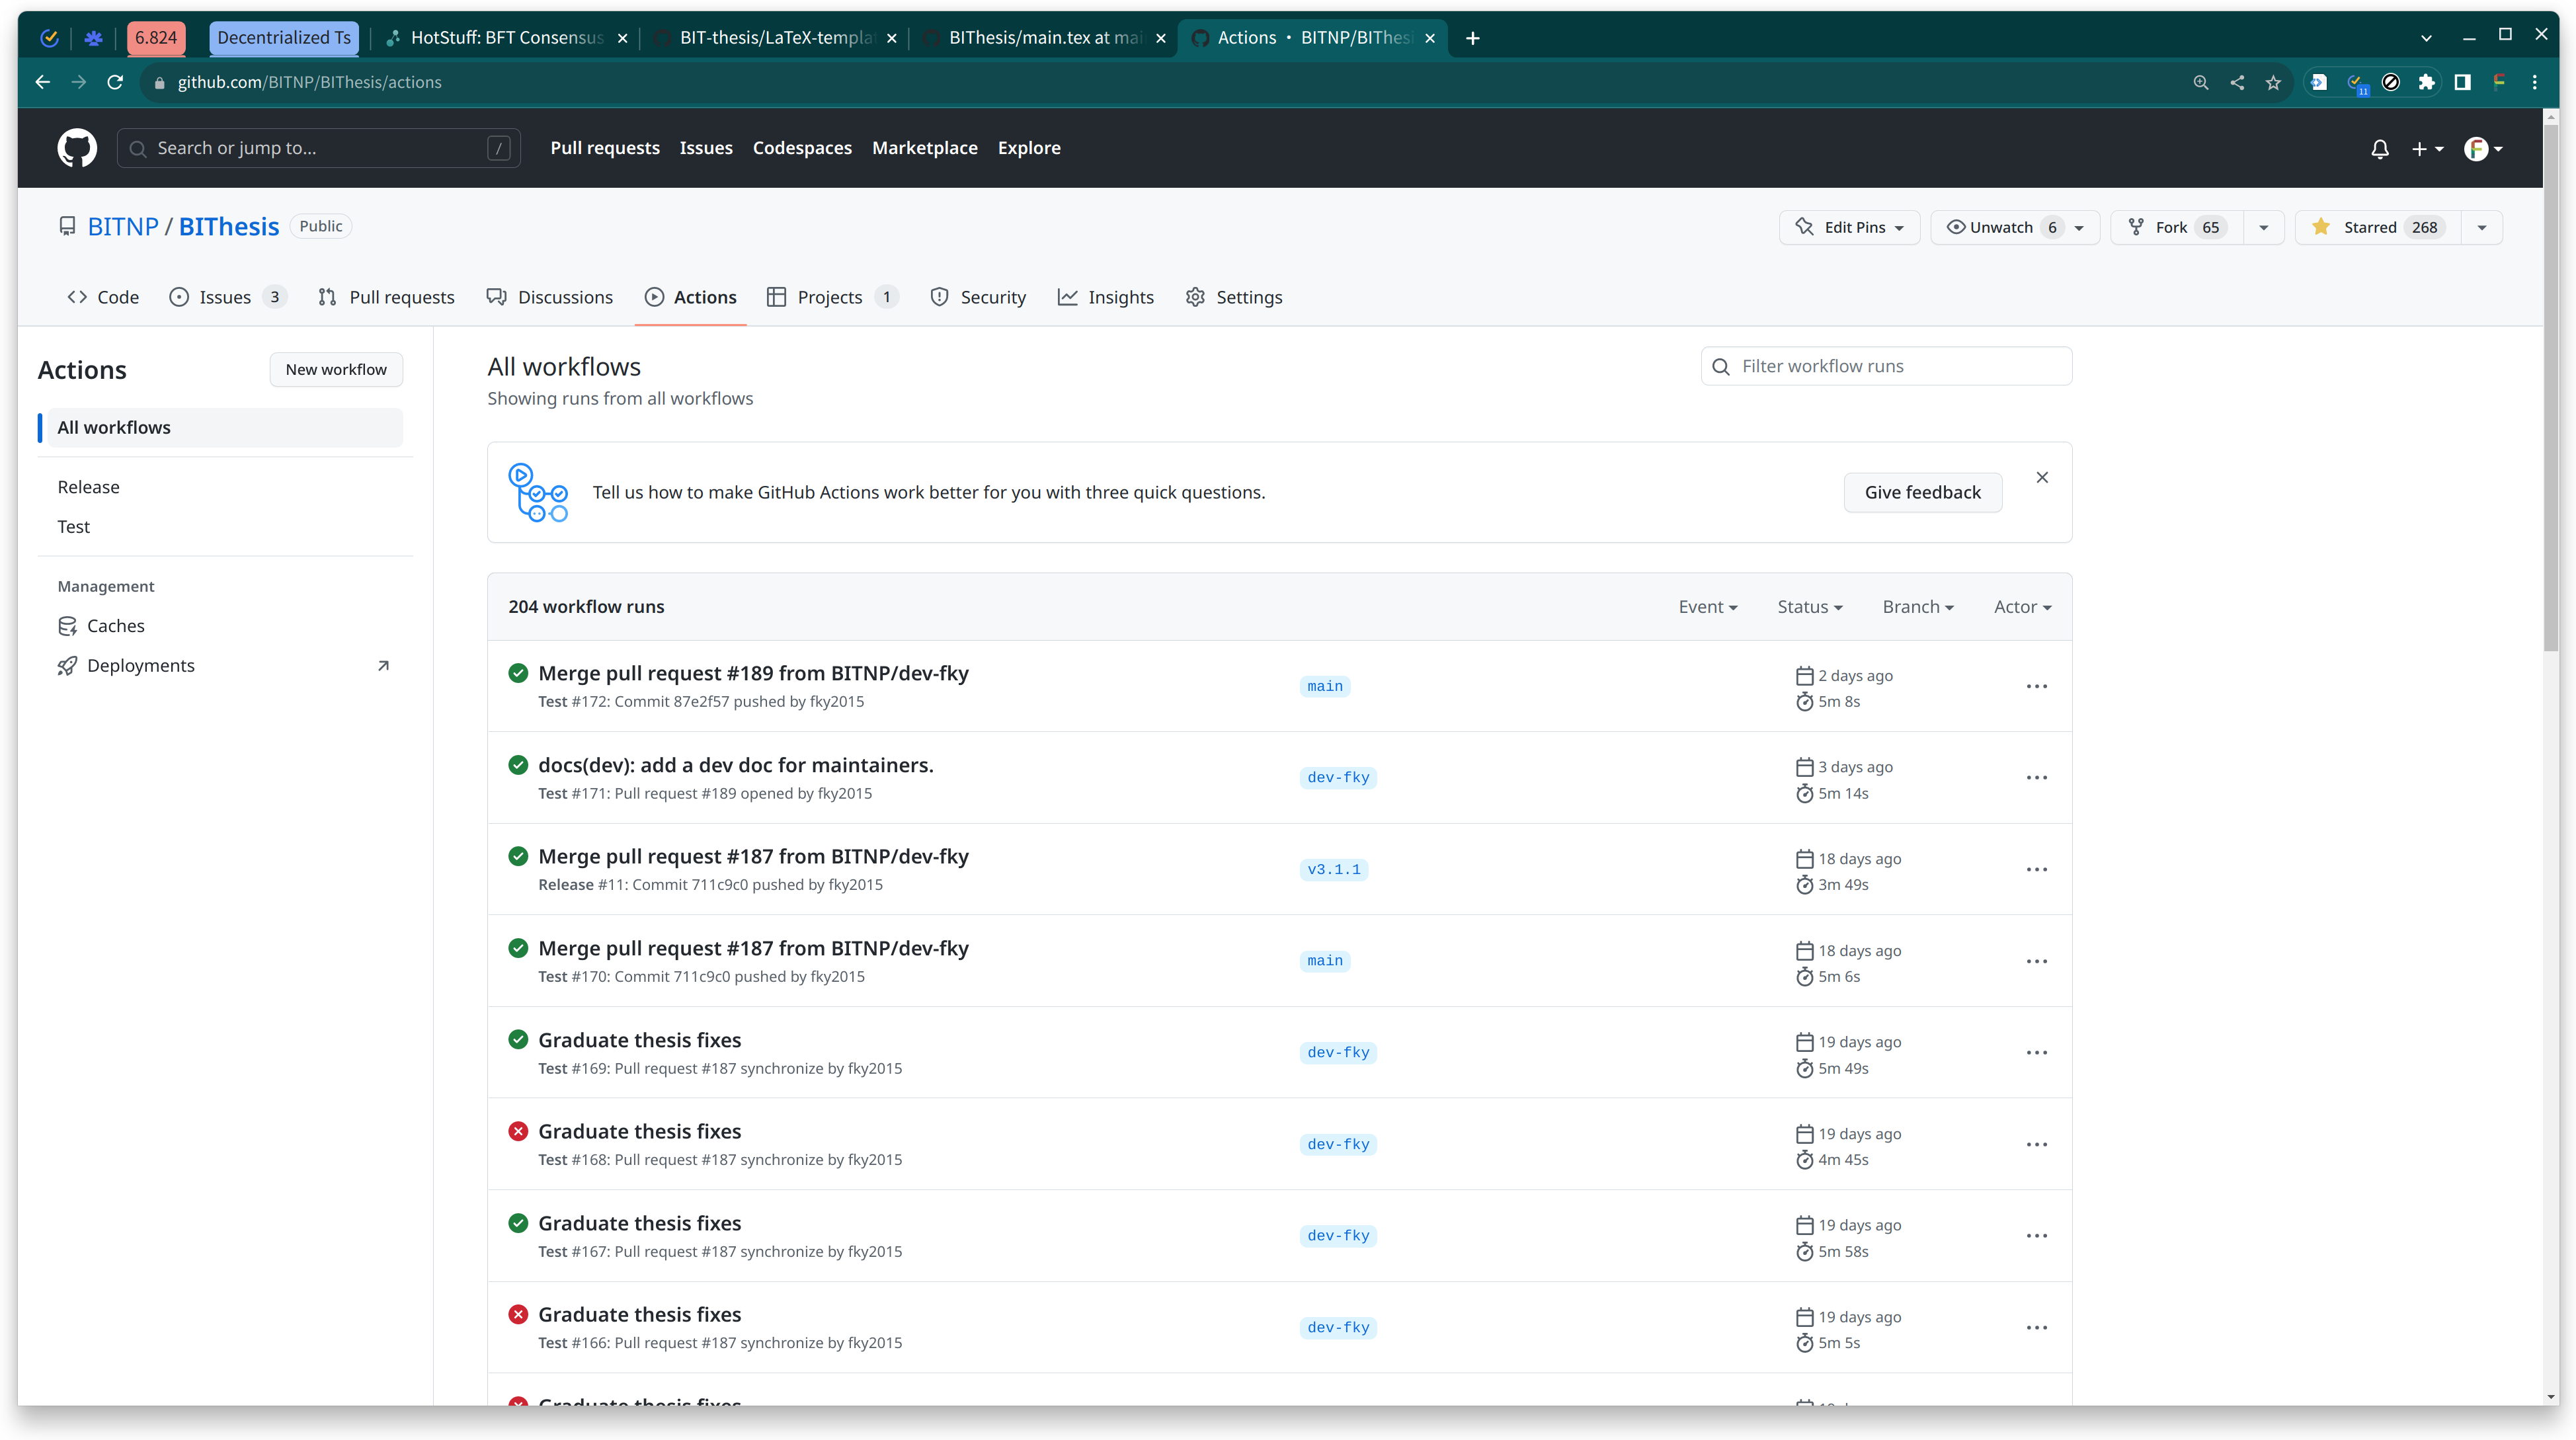
\includegraphics[width=\textwidth]{images/2.png}
      \caption{在代码合并之前的自动化测试}\label{fig:1-1}
  \end{subfigure}
  \begin{subfigure}{0.49\textwidth}
      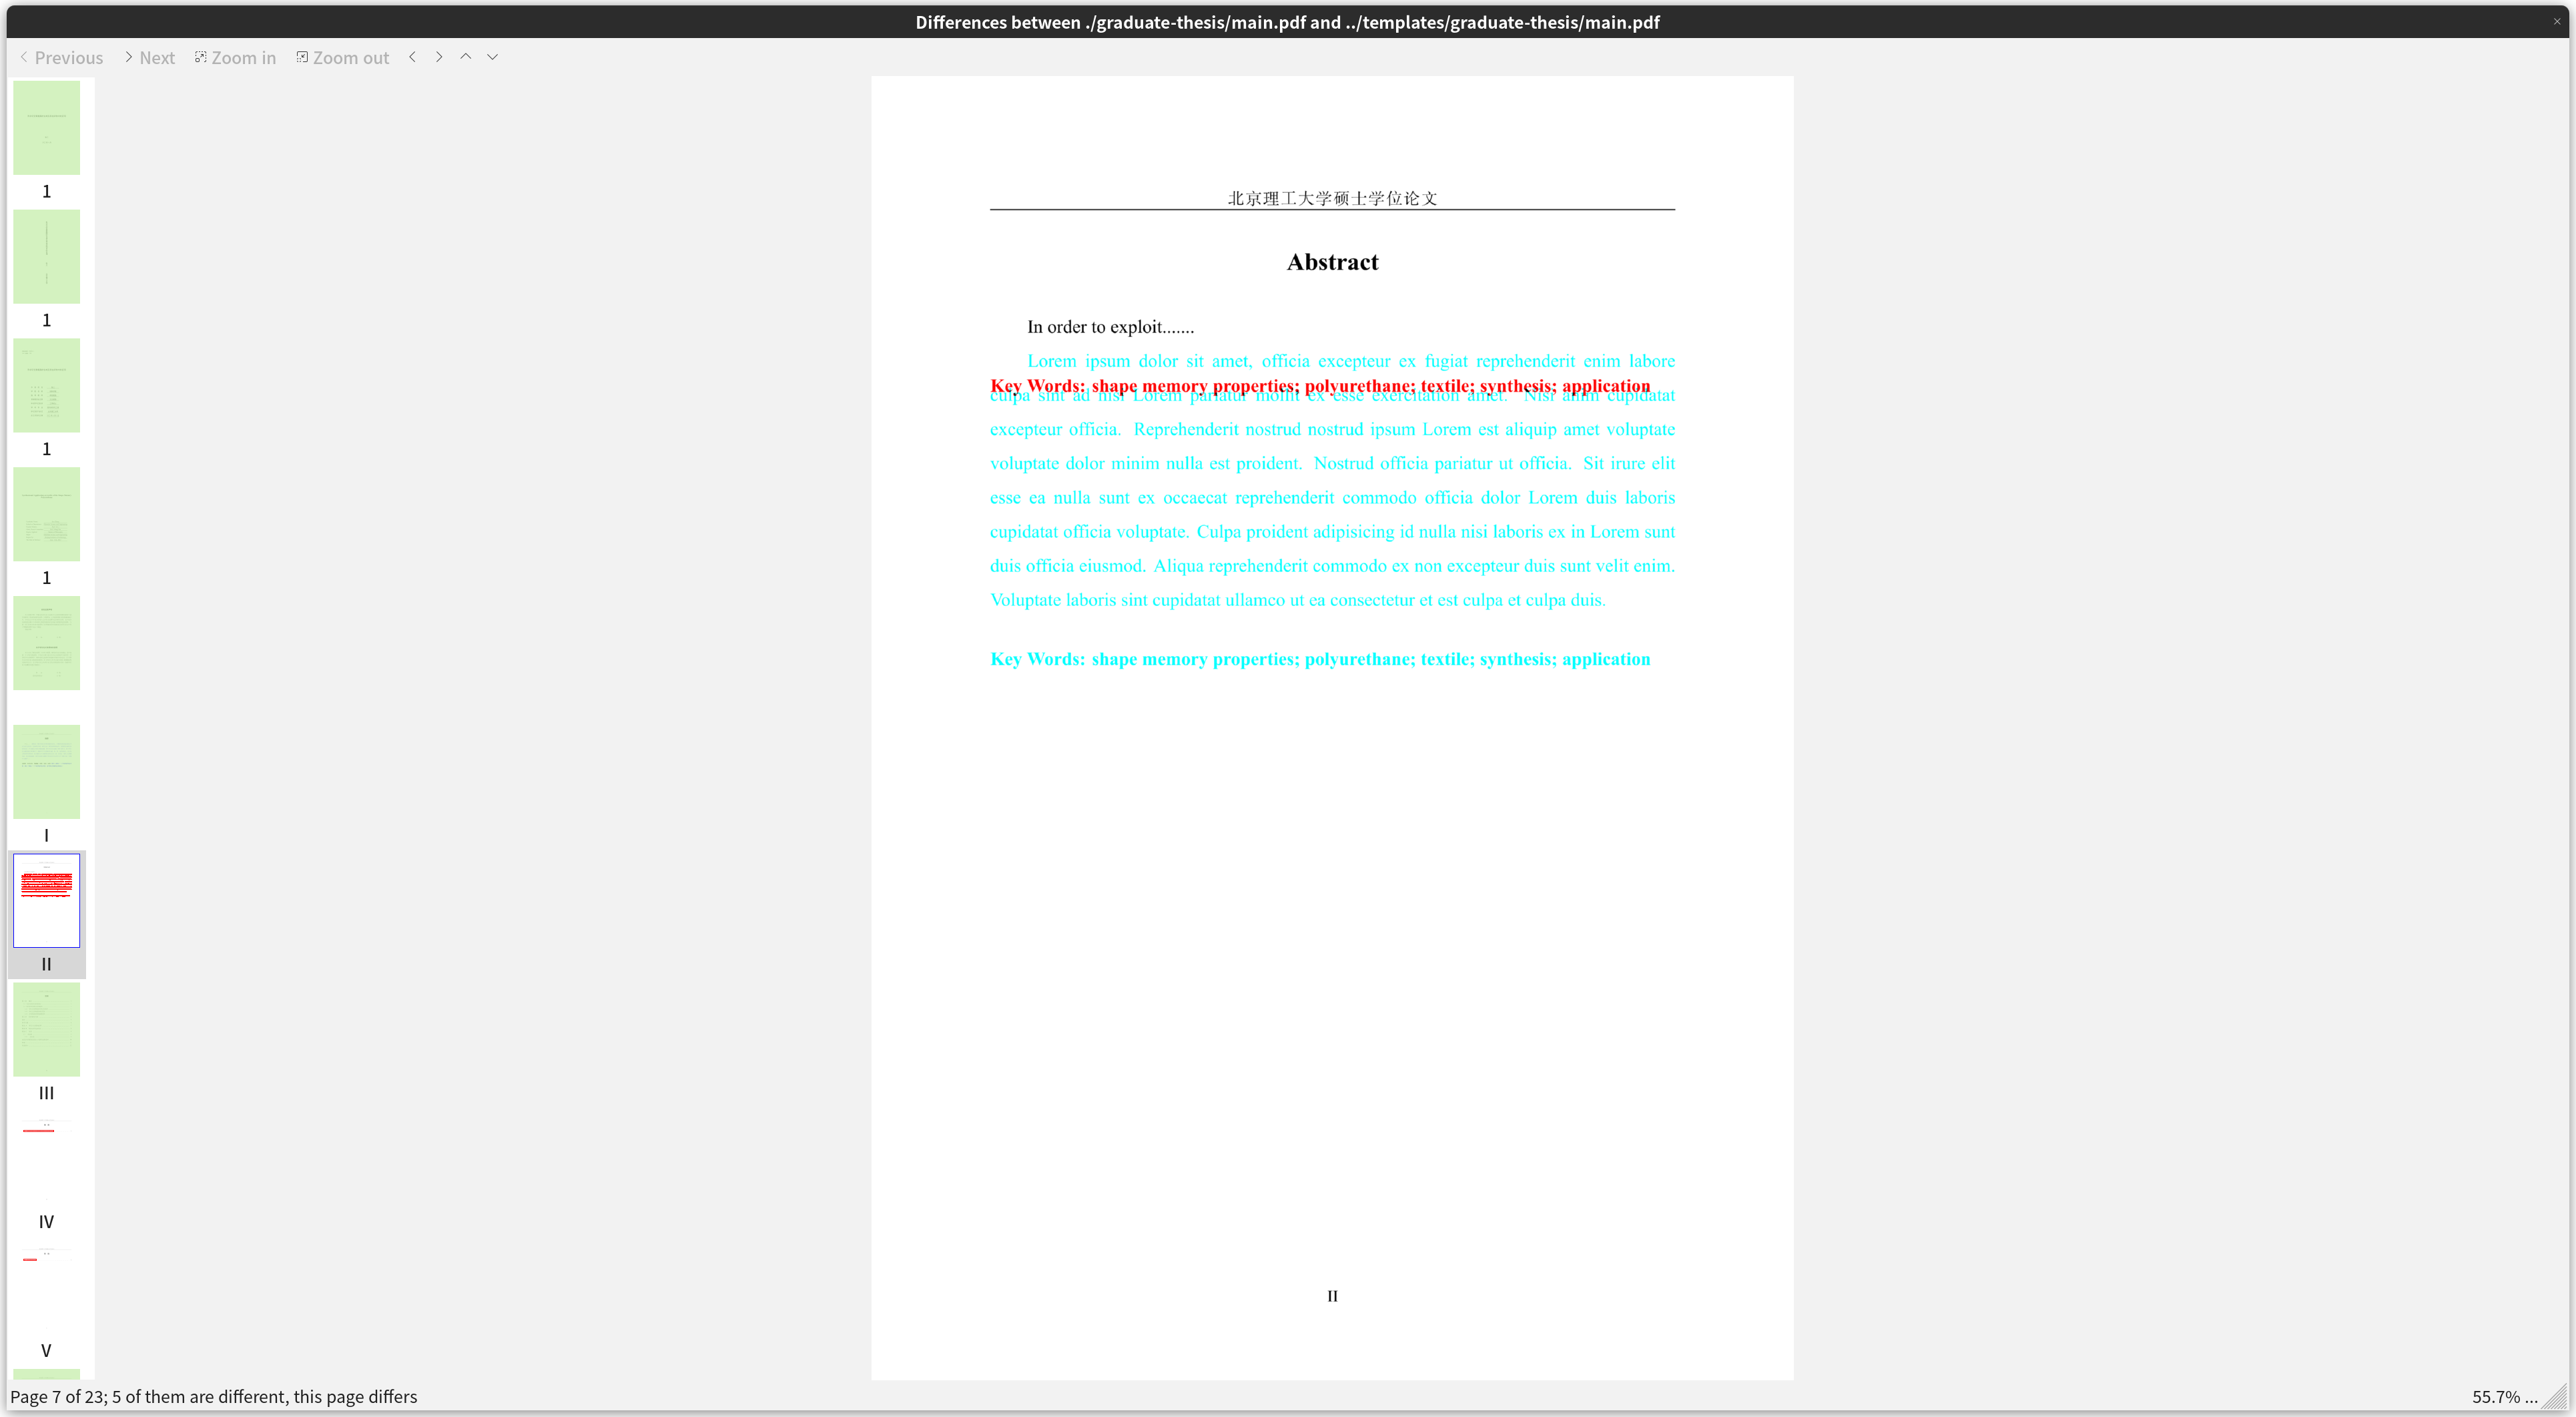
\includegraphics[width=\textwidth]{images/3.png}
      \caption{回归测试,比较两个版本的区别}\label{fig:1-2}
  \end{subfigure}
  \end{figure}
  
在发布新版本之前,BIThesis 有多种代码测试保证其正确性。
\end{frame}


\begin{frame}[c]
  \frametitle{BIThesis 的维护以及其他服务}
  \framesubtitle{规范的版本发布流程}

\begin{figure}
  \begin{center}
    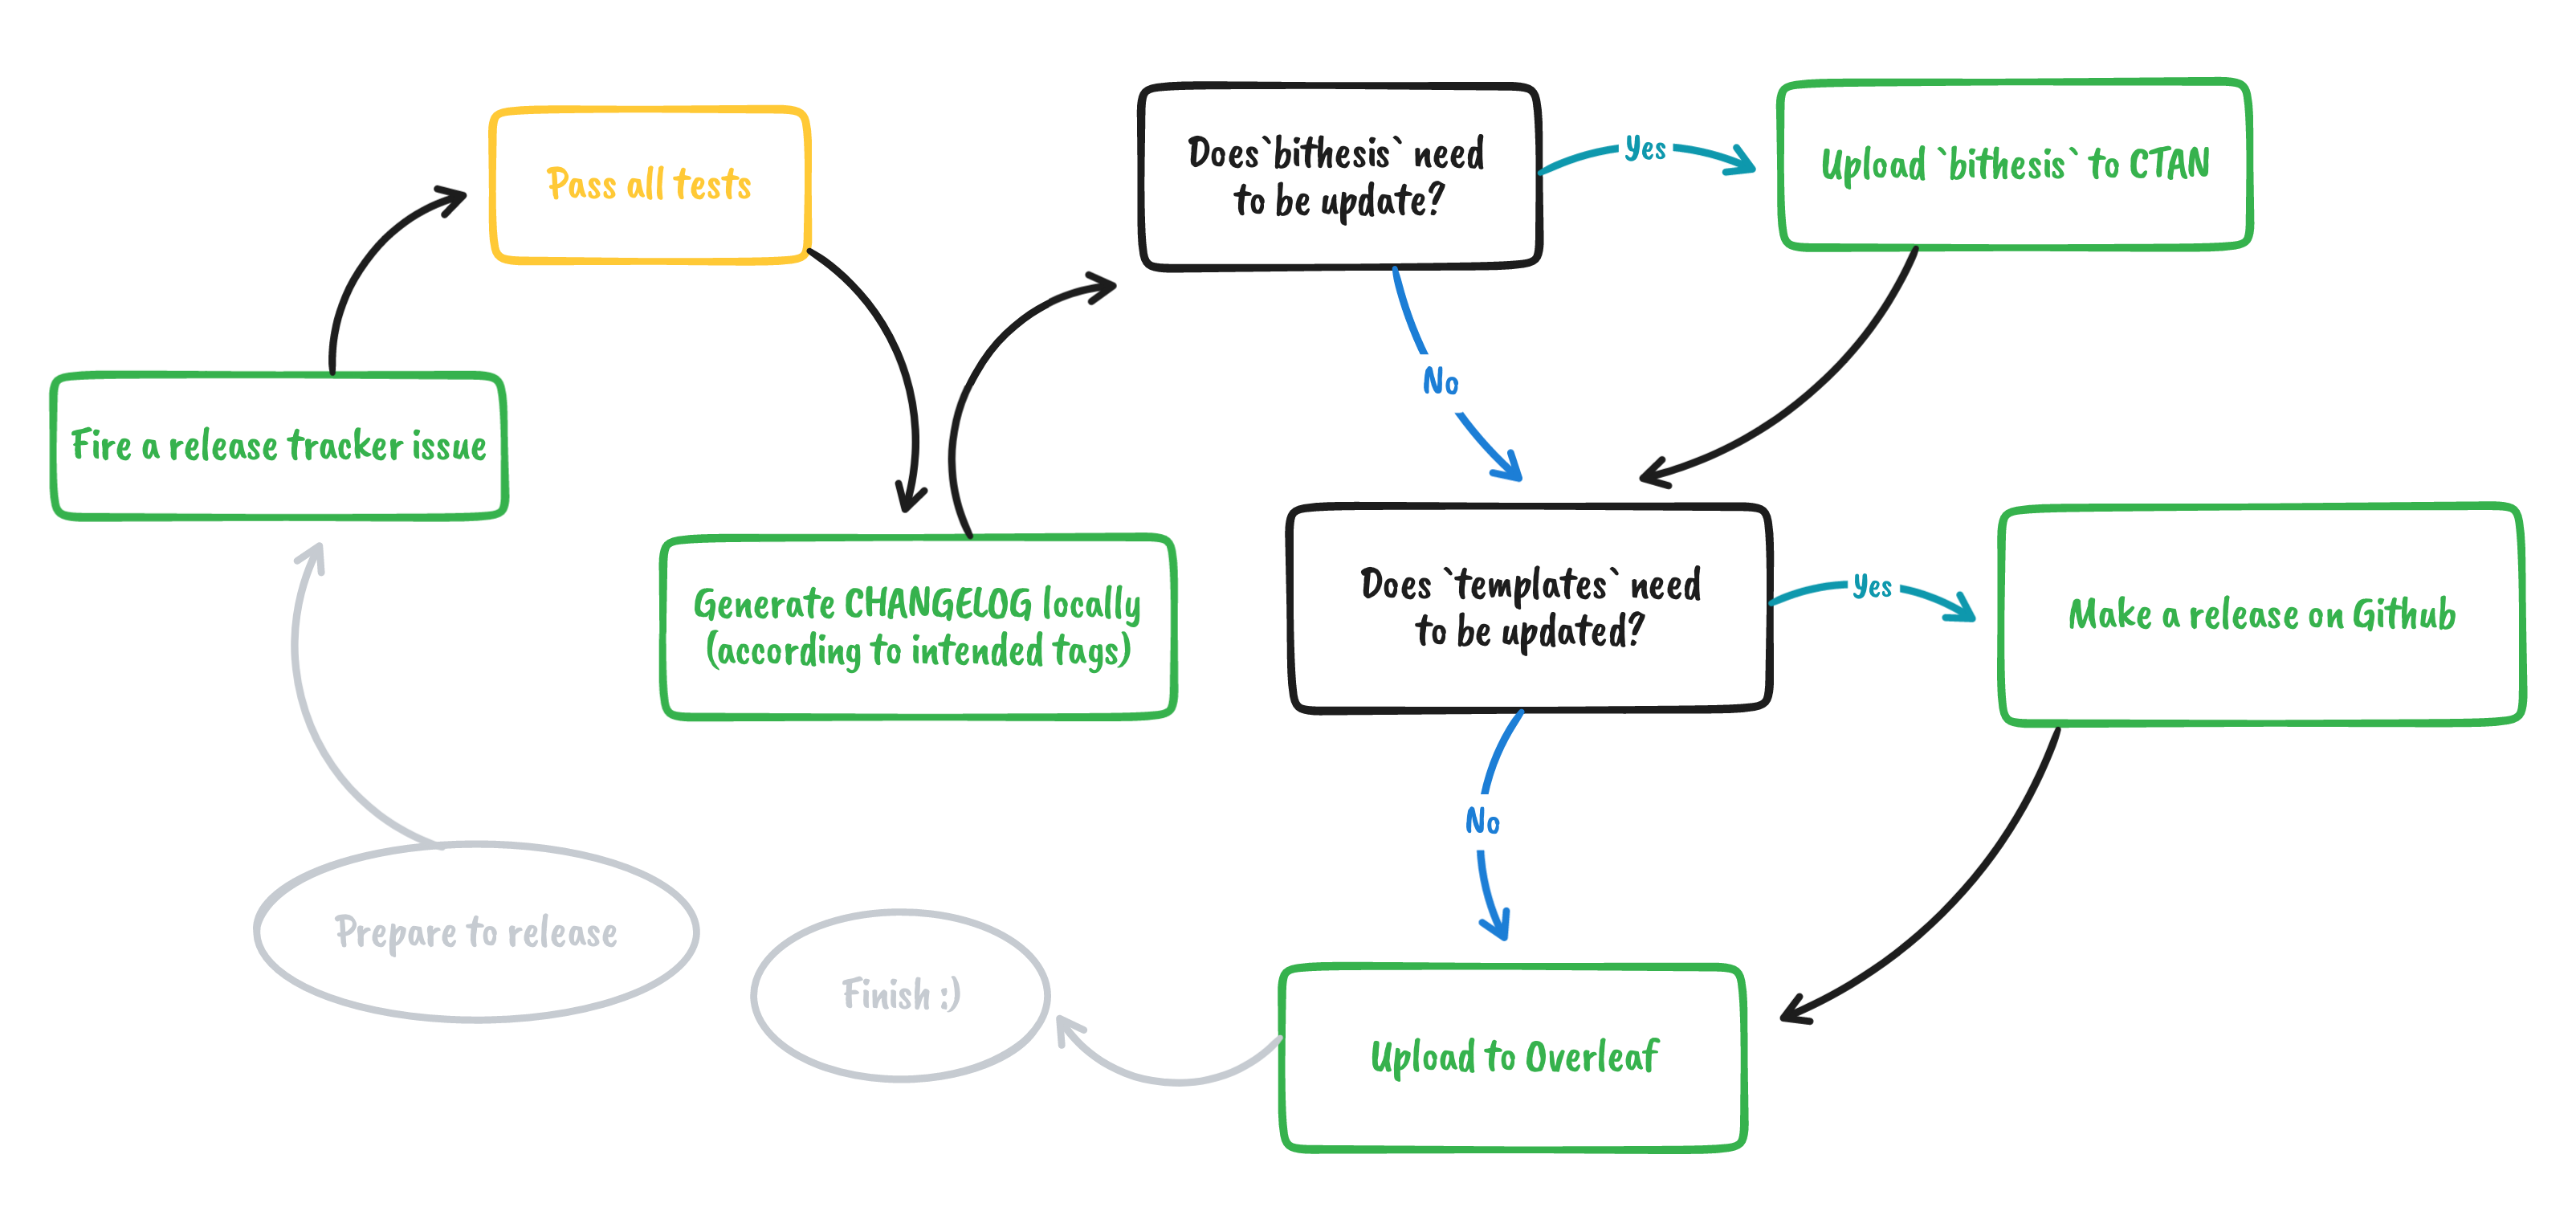
\includegraphics[width=0.6\textwidth]{images/release_workflow.png}
  \end{center}
\end{figure}

采用语义化本版号 (例如 |v3.3.1|) 不影响原有用户的使用。
在新版本发布的时候,我们会同步更新包括 CTAN, Overleaf, Github Releases 在内多个平台的版本,
保证通过各个方式使用的用户都能获得最新的代码。

\end{frame}

\begin{frame}[c]
  \frametitle{BIThesis 的维护以及其他服务}
  \framesubtitle{使用、交流方式}

  \begin{itemize}
    \item 用户可以通过使用手册了解模板的各个参数的使用方式。
    \item 用户可以通过 Github Issues 提交 Bug 或者建议。
    \item 可以加入 QQ 交流群进行讨论或者咨询。
  \end{itemize}
\end{frame}


\begin{frame}[c]

  谢谢!
  
\end{frame}

\end{document}
